\chapter{Low-Resource Data-to-Text Generation}
\label{chap:low-res}


In this chapter, we introduce three approaches for low-resource \ac{d2t} generation based on \acp{plm}. By \emph{low-resource}, we mean using as little data as possible for generating fluent and accurate text. We develop approaches that leverage the general-domain pretraining of \acp{plm} in order to generate texts in domains with thousands, hundreds, or even zero training examples.

The data we focus on are \acs{rdf} (\Acl{rdf}) triples from factual knowledge graphs and meaning representations in dialogue systems. The main feature of these kinds of data is that we always want to verbalize the whole input. For larger data, we would need a separate content selection component, but our approaches are generalizable to other kinds of data which fulfill this requirement.

The simplest setting, presented in \autoref{sec:finetuning}, consists of finetuning a pretrained transformer encoder-decoder model. For finetuning the model, we need approximately thousands of in-domain examples. We show that this baseline is powerful, achieving competitive results on a shared task for generating knowledge graph descriptions. On top of that, we show that this approach generalizes to other languages than English, namely Russian.

In \Cref{sec:iterative,sec:pipeline}, we then present approaches which can generate texts with even \emph{more limited amount} of in-domain training examples. Our key idea is to use a \ac{plm} only as a tool for improving text fluency \emph{regardless of the content}, and delegating (possibly crude and basic, but factually correct) verbalization of the content to other, simpler tools. \autoref{sec:iterative} shows an approach using a text-editing model trained on iteratively fusing simple templates, which has a limited vocabulary focused on sentence fusion. The limited vocabulary and training objective pushes the model towards generating factually correct sentences. In \autoref{sec:pipeline}, we also add an ordering and aggregation step for generating more fluent texts. For each of these steps, we can train a \ac{plm} entirely on general-domain operations, reducing the need for in-domain examples to zero.

% \section{Motivation}
% \label{sec:low-res-mot}
\section{Finetuning PLMs}
\label{sec:finetuning}

\begin{refbox}
    This section is based on the paper \emph{Train Hard, Finetune Easy: Multilingual Denoising for RDF-to-Text Generation} \cite{kasnerTrainHardFinetune2020}, joint work with Ondřej Dušek, published in the Proceedings of the 3rd International Workshop on Natural Language Generation from the Semantic Web (WebNLG+) at INLG 2020.
\end{refbox}


We introduce a simple approach for generating knowledge graph descriptions. Our approach is based on finetuning a multi-lingual \ac{plm} on linearized graphs and the accompanying human-written descriptions from the WebNLG dataset. In the WebNLG+ Shared Task, our model placed in the first third of the leaderboard for English and first or second for Russian on automatic metrics, and in the best or second-best system cluster on human evaluation.

\subsection{WebNLG+ Shared Task}
\label{sec:webnlgp}
The WebNLG Challenge 2020\footnote{\url{https://synalp.gitlabpages.inria.fr/webnlg-challenge/challenge_2020/}} (WebNLG+; \citealp{ferreira20202020}) was the second edition of the shared task in graph-to-text generation. The task was based on the WebNLG dataset, which contains subgraphs from the DBpedia knowledge graph. Each subgraph is described by a set of \ac{rdf} triples and accompanied with crowdsourced text descriptions (see \autoref{sec:datasets}). On top of the original challenge \cite{gardentWebNLGChallengeGenerating2017}, WebNLG+ included a separate track of generating texts in Russian, in which we also participated.


\subsection{Problem Formulation}
\label{sec:mbart}
Our input is a set of \ac{rdf} triples $x \in X$, where each triple $x = (s, p, o)$ describes the relation $p$ between the entities $s$ and $o$ in the knowledge graph. Our target output $Y$ is a fluent and semantically accurate natural language description of $X$.


We formulate the task as \emph{sequence-to-sequence} generation. First, we linearize the input sequence in the default order. We select two arbitrary separator tokens: one to delimit the contituents of the triple and another to delimit individual triples. Using the linearized sequence as an input and the target text, we finetune a pretrained encoder-decoder model using the cross-entropy objective (see \autoref{sec:transformer}). We use the finetuned model to generate the target texts using autoregressive decoding (see Algorithm~\ref{alg:decoding}).

% 


\subsection{Implementation}
\paragraph{Data Preprocessing} We use the provided XML WebNLG data reader\footnote{\url{https://gitlab.com/webnlg/corpus-reader}} to load and linearize the triples. For each triple, we use the \texttt{flat\_triple()} method which converts each triple into the ``\texttt{s $\vert$ p $\vert$ o}'' string, using a pipe (``$\vert$'') as a separator. We use another token not present in the training data (``$\blacktriangleright$'') for delimiting individual triples to avoid extending the model vocabulary.\footnote{Our choice of the separators is arbitrary, as we will adapt the model to account for our separators.
    % Works such as \TODO{cite} or \TODO{cite} show that the choice of separators is not important.
} We linearize the triples in their default order. For the input to the model, we tokenize the data using SentencePiece tokenizer \citep{kudo2018sentencepiece} trained on the training dataset, using a vocabulary of 250,000 subword tokens.

\paragraph{Model}
We use mBART \cite{liuMultilingualDenoisingPretraining2020}, a multilingual \ac{plm} based on BART, a transformer model pretrained on text denoising (see \autoref{sec:plms}).
% In pretraining, the noise function of mBART replaces text spans of arbitrary length with a mask token (35\% of the words in each instance) and permutes the order of sentences. 
The model uses 12 layers for the encoder and 12 layers for the decoder ($\sim$680M parameters), and it is pretrained on the large-scale CC25 corpus extracted from Common Crawl, which contains data in 25 languages \citep{wenzek2020ccnet}.



\paragraph{Training} We finetune the pre-trained \texttt{mbart.CC25} model from the \textsc{fairseq} toolkit \citep{ott2019fairseq} using the default parameters.\footnote{We use dropout 0.3, attention dropout 0.1, and 1024 tokens per batch. We set the initial learning rate to 0.0003 and use polynomial decay with 2500 warmup steps. We train the model using the Adam optimizer \cite{kingma2014adam} with $\beta_1=0.9, \beta_2=0.98$ and $\varepsilon=1e-06$. For the full setup, see \url{https://github.com/facebookresearch/fairseq/tree/main/examples/mbart}.} We change the total number of updates from 40k to 10k to reflect the smaller size of our data. We train a separate version of mBART for each language: $\text{mBART}_{\text{en}}$ on English inputs and English outputs, and $\text{mBART}_{\text{ru}}$ on English inputs and Russian outputs.



\subsection{Results}

\begin{table*}[t]
    \footnotesize
    \centering
    \begin{tabular}{@{}lp{12.7cm}@{}}
        \textbf{input}    & \texttt{Piotr\_Hallmann | weight | 70.308 }  $\blacktriangleright$ \texttt{ Piotr\_Hallmann | birthDate | 1987-08-25} \\
        \textbf{out (en)} & Born on August 25th 1987, Piotr Hallmann has a weight of 70.308.                                                      \\
        \midrule
        \textbf{in}       & \texttt{Ciudad\_Ayala | populationMetro | 1777539}                                                                    \\
        \textbf{out (en)} & The population metro of Ciudad Ayala is 1777539.                                                                      \\
        \midrule
        \textbf{in}       & \texttt{Bakewell\_tart | ingredient | Frangipane}                                                                     \\
        \textbf{out (ru)} & Франжипан - один из ингредиентов тарта Бейквелл.                                                                      \\[0.1cm]
        \textbf{transcr.} & Franzhipan - odin iz ingredientov tarta Bejkvell.                                                                     \\
        \textbf{transl.}  & Frangipane is one of the ingredients of the Bakewell tart.                                                            \\
    \end{tabular}
    \caption{Example outputs from the mBART model(s) finetuned for \ac{rdf}-to-text generation. (1) The model can work with unseen entities, dates and numbers. (2) The model is quite robust to unseen properties, such as \texttt{populationMetro}. However, the surface form of the property deviates too much from its meaning and the sentence is incorrect. (3) The model trained on Russian targets can use English data to form sentences in Russian, transcribing the entities to Cyrillic.}
    \label{tab:mbart:examples}
\end{table*}

We report on WebNLG automatic and human evaluation results, as well as our own error analysis.

\paragraph{Automatic Metrics}
The results of our approach for English are shown in \autoref{tab:mbart:results-en}, comparing to the baseline.
% \footnote{See \url{https://gerbil-nlg.dice-research.org/gerbil/webnlg2020results} for full results.} 
We can see that our approach beats the baseline in all metrics and places in the first third of the submissions. While it does lose performance on unseen categories, the drop is not as dramatic as for many other competing approaches.

The results for Russian are shown in \autoref{tab:mbart:results-ru}. There were fewer submissions for Russian, and our system not only beats the baseline by a large margin (as did all competing submissions), but it is able to rank first in 2 metrics out of 4 (BLEU, BERTScore) and second in the remaining ones.

\paragraph{Human Evaluation}

The challenge organizers ran a human evaluation campain, where annotators were asked to rate the texts for data coverage, relevance, correctness, text structure and fluency.  Each criterion has been rated with a number in the range from 0 (completely disagree) to 100 (completely agree). The scores were clustered into groups (1-5; 1 being the best) among which there are no statistically significant differences according to the Wilcoxon rank-sum test \citep{wilcoxon1992individual}.

Our systems placed in the top clusters (1 or 2) for both English and Russian. For English, our $\text{mBART}_{\text{en}}$ system ranks first for all the categories in \textit{seen domains}, and first or second in \textit{unseen entities} and \textit{unseen domains}. In total, our English system achieved rank 1 for relevance, correctness and text structure, and rank 2 for data coverage and fluency. For Russian, our $\text{mBART}_{\text{ru}}$ system ranks second for correctness and first in all other categories.


\begin{table*}[t]
    \footnotesize\centering
    \begin{tabular}{llcccccccccc}\toprule
                                     &          & \multicolumn{2}{c}{\bf BLEU} & \multicolumn{2}{c}{\bf METEOR} & \multicolumn{2}{c}{\bf ChrF++} & \multicolumn{2}{c}{\bf BERTScore} & \multicolumn{2}{c}{\bf BLEURT}                                     \\\midrule
        \multirow{2}{*}{All}         & Ours     & 50.34                        & (10)                           & 0.398                          & (8)                               & 0.666                          & (8)  & 0.951 & (8)  & 0.57 & (8)  \\
                                     & Baseline & 40.57                        & (14)                           & 0.373                          & (15)                              & 0.621                          & (15) & 0.943 & (14) & 0.47 & (12) \\\midrule
        \multirow{2}{*}{Seen Cat.}   & Ours     & 59.13                        & (10)                           & 0.422                          & (10)                              & 0.712                          & (9)  & 0.960 & (9)  & 0.58 & (14) \\
                                     & Baseline & 42.95                        & (31)                           & 0.387                          & (27)                              & 0.650                          & (28) & 0.943 & (31) & 0.41 & (31) \\\midrule
        \multirow{2}{*}{Unseen Cat.} & Ours     & 42.24                        & (10)                           & 0.375                          & (13)                              & 0.617                          & (10) & 0.943 & (11) & 0.52 & (10) \\
                                     & Baseline & 37.56                        & (12)                           & 0.357                          & (15)                              & 0.584                          & (15) & 0.940 & (12) & 0.44 & (12) \\\midrule
        \multirow{2}{*}{Unseen Ent.} & Ours     & 51.23                        & (4)                            & 0.406                          & (8)                               & 0.687                          & (7)  & 0.959 & (8)  & 0.63 & (8)  \\
                                     & Baseline & 40.22                        & (17)                           & 0.384                          & (15)                              & 0.648                          & (15) & 0.949 & (13) & 0.55 & (12) \\\bottomrule
    \end{tabular}
    \caption{Results of $\text{mBART}_{\text{en}}$ (all data, seen categories, unseen categories, unseen entities), compared to the baseline. The numbers in brackets show the rank of each model (out of 35 submissions) with respect to the given metric.}
    \label{tab:mbart:results-en}
\end{table*}
\begin{table*}[t]
    \footnotesize\centering
    \begin{tabular}{llcccccccc}\toprule
                 & \multicolumn{2}{c}{\bf BLEU} & \multicolumn{2}{c}{\bf METEOR} & \multicolumn{2}{c}{\bf ChrF++} & \multicolumn{2}{c}{\bf BERTScore}                               \\\midrule
        Ours     & 52.93                        & (1)                            & 0.672                          & (2)                               & 0.677 & (2)  & 0.909 & (1)  \\
        Baseline & 23.53                        & (12)                           & 0.461                          & (12)                              & 0.511 & (12) & 0.836 & (12) \\\bottomrule
    \end{tabular}
    \caption{Results of $\text{mBART}_{\text{ru}}$, compared to the baseline. The numbers in brackets show the rank of each model (out of 12 submissions) if ordered by the given metric.}
    \label{tab:mbart:results-ru}
\end{table*}

\paragraph{Manual Analysis}
To better understand the nature of errors made by our system, we manually inspected a sample of 50 outputs in each language.\footnote{Automatic back-translation to English was used to facilitate understanding of Russian.} We found factual errors in 12 English outputs, mostly concentrated along the unseen categories (\emph{Scientist}, \emph{Movie}, \emph{Musical Record}). The model tends to describe musical works and movies in terms of written works (“written”, “published” etc.), i.e., the closest seen category. There are also several swaps in roles of the entities (e.g., “is to southeast” instead of “has to its southeast”, “follows” instead of “is followed by” etc.).

In a few cases, the model hallucinates a relation not specified in the data (e.g., “born on January 1, 1934 in Istanbul” when a date of birth and current residence is given, not the birthplace) or is not able to infer background knowledge not given on the input (it talks about a dead person in the present tense).
% The swaps in roles and hallucinated relations also occured in Russian; in addition, we found a hallucinated (correct) airport name and a few forgotten ingredients for a dish from a long list. 
Factual errors in Russian were less frequent (9 sentences), which is expected as there are no unseen categories. Moreover, the system shows an impressive performance at translating entity names from the English \ac{rdf} into Russian.

We further found 10 outputs with suboptimal phrasing in English and 9 in Russian, where the model did not connect properties of the same type in a coordination (e.g., two musical genres for a record) or gave numbers without proper  units (e.g., “runtime of 89.0” or “area of 250493000000.0”).

\paragraph{Discussion}
Our solution benefits from the pretrained representations of the mBART model. Multilingual pretraining allows us to use a single architecture for both English and Russian. However, English and Russian are the two most represented languages in the mBART pre-training corpora (ca. 300 GB of data each) and the performance of our model would probably be lower with low-resource languages.

The performance of our model is also noticeably lower on categories unseen in training, and it is prone to swapping relations of entities or hallucinating relations. Even though the longest examples in the WebNLG dataset fit into the model, the length of the input sequence is still limited and the model does not generalize for inputs of arbitrary size.





\section{Iterative Template Fusion}
\label{sec:iterative}

\begin{refbox}
    This section is based on the paper \emph{Data-to-Text Generation with Iterative Text Editing} \cite{kasnerDatatoTextGenerationIterative2020}, joint work with Ondřej Dušek, published in the Proceedings of the 13th International Conference on Natural Language Generation (INLG 2020).
\end{refbox}

We present an approach for generating semantically accurate texts from structured data in low-resource settings. Our approach builds on a text-editing model trained on the task of \emph{sentence fusion}. We first transform individual data items to text using trivial templates, and iteratively improve the resulting text using the sentence fusion model, filtering, and re-ranking.  Our approach gets lower scores on lexical similarity metrics on WebNLG and E2E datasets than the state-of-the-art approaches; however, it achieves high levels of semantic accuracy due to the limited scope of the sentence fusion model and guaranteed presence of the entities. We also demonstrate that our task formulation opens up the possibility for zero-shot \ac{d2t} generation by training a model on a general-domain dataset for sentence fusion. The code for the experiments is available on Github.\footnote{\url{https://github.com/kasnerz/d2t_iterative_editing}}


\subsection{Motivation}
\label{sec:text-editing}
Our goal is to improve the semantic accuracy \ac{d2t} generation. Other works have pursued this goal, e.g., by adapting the decoding algorithm \cite{tianStickingFactsConfident2020}, improving robustness of the model by injecting noise in its hidden states \cite{kedzie_good_2019}, or self-training with a natural language understanding model \cite{nieSimpleRecipeReducing2019}. Our approach is inspired by the systems which use a \emph{generate-then-rerank} approach \citep{dusekSequencetoSequenceGenerationSpoken2016,juraska_deep_2018}, e.g. using a classifier \cite{harkousHaveYourText2020}, to filter incorrect outputs.

To generate outputs with sufficient semantic accuracy for the filtering step, we take advantage of three facts: (1) we can lexicalize individual data items using trivial templates, (2) concatenating the lexicalizations tends to produce an unnatural sounding but semantically accurate output, and (3) a \ac{plm} trained on improving the output fluency can be used for combining the lexicalizations.

% \textsc{LaserTagger} \cite{malmi2019lasertagger}, which we use in our approach, is a sequence tagging model based on the transformer architecture with BERT \cite{devlinBERTPretrainingDeep2019} as the encoder backbone. Other recent text-editing models without a pre-trained backbone include EditNTS \citep{dong} and Levenshtein Transformer \citep{gu2019levenshtein}.

% Concurrently with our work, \citet{kale2020few} explored using templates for dialogue response generation. %\ODdel{Unlike our work,} 
% They use the sequence-to-sequence T5 model \citep{raffel2019exploring} to generate the output text from scratch instead of iteratively editing the intermediate outputs, which leaves less control over the model.


\subsection{Our Approach}
\label{sec:text-editing-exp}
We focus on data structured as \ac{rdf} triples.\footnote{Later, we also trivially extend our approach to key-value pairs.} In our approach, we start from single-triple templates and iteratively fuse them into the resulting text while filtering and reranking the results. We first detail the main components of our system (template extraction, sentence fusion, \ac{plm} scoring) and then give the overall description of the generation algorithm.

\begin{figure*}[t]
    \centering
    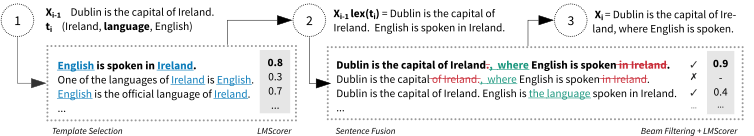
\includegraphics[width=\textwidth]{img/d2t_text_editing}
    \caption{A single iteration of our algorithm for iterative \ac{d2t} generation. In Step 1, the template for the triple is selected and filled. In Step 2, the sentence is fused with the template. In Step 3, the result for the next iteration is selected from the beam by filtering and language model scoring.}\label{fig:iterative:alg}
\end{figure*}



\paragraph{Template Extraction}
We collect a set of templates for each unique predicate. We use two approaches: (a) handcrafting the template manually for each predicate in the training set, and (b) automatically extracting the template from the lexicalizations of the examples  in the training set. For unseen predicates, we add a single fallback template: \textit{The <predicate> of <subject> is <object>.}


\paragraph{Sentence Fusion}
We train a model for the task of \emph{sentence fusion}, i.e., combining sentences into a coherent text \cite{barzilay2005sentence}.
%We train an independent in-domain sentence fusion model for each dataset. 
To construct the training data for the model, we select pairs of examples $(X, X')$ and their corresponding text descriptions $(Y, Y')$ from the original training set such that the examples consist of $(k, k+1)$ triples and have $k$ triples in common. This leaves us with an extra triple $x_{k+1}$ present only in $X'$. For each training example, we use the concatenated sequence $Y \mathrm{lex}(x_{k+1})$ as a source and the sequence $Y'$ as a target, where $\mathrm{lex}(x_{k+1})$ denotes lexicalizing the triple $x_{k+1}$ using an appropriate template.
As a result, the model learns to integrate $Y$ and $x_{k+1}$ into a single coherent expression.


\paragraph{PLM Scoring} For re-ranking the text, we use an additional component for computing text fluency, which we refer to as \textsc{LMScorer}.
As described in \autoref{sec:evaluation}, we use perplexity of the text under a a \ac{plm}, computing the score of the output text $Y$ composed of tokens $(y_1, \ldots, y_n)$ as a geometric mean of the token conditional probability:
\begin{align}
    \operatorname{score}(Y) = \Bigg( \prod_{i=1}^{n}{P(y_i|y_1, \ldots, y_{i-1})} \Bigg)^{\frac{1}{n}}.
\end{align}




\paragraph{Generation Algorithm}
The input of the algorithm (\autoref{fig:iterative:alg}) is a set of $T$ ordered triples. First, we lexicalize the triple $x_0$ to get the output text $Y_0$ by filling the available templates and using the template with the best score from \textsc{LMScorer}.
% This promotes templates which sound more natural for particular values.
In each of the following steps $i=(1, \ldots, T-1)$, we lexicalize the triple $x_i$ and concatenate it with $Y_{i-1}$.  For improving the fluency of the text, we use the sentence fusion model with beam search to produce $k$ hypotheses. We filter and re-rank the hypotheses, getting $Y_{i}$ (see the next paragraph), and proceed to the next step. The output of the algorithm is the text $Y_{T-1}$ from the final step.


\paragraph{Filtering and Re-ranking} In each decoding step, we remove hypotheses in the beam missing any entity from the input data using a simple heuristic based on string matching. Next, we rescore the remaining hypotheses in the beam with \textsc{LMScorer} and set the hypothesis with the best score as $Y_{i}$. In case there are no sentences left in the beam after the filtering step, we let $Y_{i}$ be the text in which the lexicalized $x_i$ is appended after $Y_{i-1}$ without sentence fusion, ensuring the semantic accuracy of the text.

%For the E2E dataset, we first try to find a pair of predicates for which there is a template extracted from the data, and only use the handcrafted templates for the single predicates in the subsequent steps. 
%The final beam filtering step is a simple heuristic, checking if all entities from the input triples are present in the output.


\subsection{Implementation}


\begin{table}[t]
    \centering\footnotesize
    \begin{tabular}{lllll}
        \textbf{dataset} & \textbf{method} & \textbf{predicate}          & \textbf{example \#1}                            & \textbf{example \#2}                     \\\midrule
        WebNLG           & extracted       & \texttt{foundedBy}          & \textit{$o$ was the founder of $s$.}            & \textit{$s$ was founded by $o$.}         \\
        E2E              & extracted       & \texttt{area}+\texttt{food} & \textit{$s$ offers $o_2$ cuisine in the $o_1$.} & \textit{$s$ in $o_1$ serves $o_2$ food.} \\
        E2E              & manual          & \texttt{near}               & \textit{$s$ is located near $o$.}               & \textit{$o$ is close to $s$.}
    \end{tabular}
    \caption{Examples of templates we used in our experiments. The templates for the single predicates in the WebNLG dataset and the pairs of predicates in the E2E dataset are extracted automatically from the training data; the templates for the single predicates in E2E are created manually.}
    \label{tab:iterative:templates_ex}
\end{table}


\paragraph{Template Extraction} We experiment with the WebNLG and E2E datasets (see \autoref{sec:datasets}). For WebNLG, we extract the templates from the training examples containing only a \textit{single} triple. In the E2E dataset, there are no such examples; therefore we first extract the templates for \textit{pairs} of predicates, using them as a starting point for the algorithm in order to leverage the lexical variability in the data (manually filtering out the templates with semantic noise), and we also create a small set of templates for each \textit{single} predicate manually, using them in the subsequent steps of the algorithm.\footnote{In the E2E dataset, the data is in the form of key-value pairs. We transform the data to \ac{rdf} triples by using the name of the restaurant as a \textit{subject} and the rest of the pairs as \textit{predicate} and \textit{object}. This creates \textit{n-1} triples for \textit{n} pairs.} See \autoref{tab:iterative:templates_ex} for examples of templates we used in our experiments.

\paragraph{Sentence Fusion Model} We base our sentence fusion model on the text-editing model \textsc{LaserTagger} \cite{malmi2019lasertagger}. \textsc{LaserTagger} generates outputs by tagging inputs with edit operations (\texttt{KEEP} a token, \texttt{DELETE} a token, and \texttt{ADD} a phrase before the token), which makes it suitable for tasks where the output highly overlaps with the input. An important feature of \textsc{LaserTagger} is the limited size of its vocabulary, which consists of $l$ most frequent (possibly multi-token) phrases used to transform inputs to outputs in the training data. After the vocabulary is precomputed, all infeasible examples in the training data are filtered out. At the cost of limiting the number of training examples, this filtering makes the training data cleaner by removing outliers. The limited vocabulary also makes the model less prone to hallucinations errors.

\paragraph{LMScorer} As the \textsc{LMScorer} backend, we use the pre-trained GPT-2 language model \citep{radford2019language} from the Transformers repository\footnote{\url{https://github.com/huggingface/transformers}} \citep{wolf2019HuggingFacesTS}. We compute the perplexity scores using the \textit{lm-scorer}\footnote{\url{https://github.com/simonepri/lm-scorer}} package.





\begin{table*}[t]% \begin{adjustbox}{max width=\textwidth}
    \centering\footnotesize
    \begin{tabular}{lcccc<{\hspace{2mm}}c>{\hspace{2mm}}cccc} \toprule
                         & \multicolumn{4}{c}{\bf WebNLG} &            & \multicolumn{4}{c}{\bf E2E}                                                                                                                                                                          \\
        \cmidrule{2-5} \cmidrule{7-10}
                         & {\it BLEU}                     & {\it NIST} & \hspace{-1mm}{\it METEOR}\hspace{-1mm} & \hspace{-1mm}{\it ROUGE$_L$}\hspace{-1mm} &  & {\it BLEU} & {\it NIST} & \hspace{-1mm}{\it METEOR}\hspace{-1mm} & \hspace{-1mm}{\it ROUGE$_L$}\hspace{-1mm} \\
        {\bf baseline}   & 0.277                          & 6.328      & 0.379                                  & 0.524                                     &  & 0.207      & 3.679      & 0.334                                  & 0.401                                     \\
        {\bf zero-shot } & 0.288                          & 6.677      & 0.385                                  & 0.530                                     &  & 0.220      & 3.941      & 0.340                                  & 0.408                                     \\
        {\bf w/fusion }  & 0.353                          & 7.923      & 0.386                                  & 0.555                                     &  & 0.252      & 4.460      & 0.338                                  & 0.436                                     \\
        {\bf SFC }       & 0.524                          & -          & 0.424                                  & 0.660                                     &  & 0.436      & -          & 0.390                                  & 0.575                                     \\
        {\bf T5 }        & 0.571                          & -          & 0.440                                  & -                                         &  & -          & -          & -                                      & -                                         \\ \bottomrule
    \end{tabular}
    \caption{Results of automatic metrics on the WebNLG and E2E test sets. The comparison is made with the results from the papers on the Semantic Fidelity Classifier (SFC; \citealp{harkousHaveYourText2020}) and the finetuned T5 model (T5; \citealp{kaleTexttoTextPreTrainingDatatoText2020}), state-of-the-art approaches at that time.}
    \label{tab:results}
    % \end{adjustbox}
\end{table*}



\subsection{Experiments}
\paragraph{Base Experiments} As a \emph{baseline}, we generate the best templates according to \textsc{LMScorer} without applying the sentence fusion (i.e., always using the fallback). For the \emph{sentence fusion} experiments, we use \textsc{LaserTagger} with the autoregressive decoder with a beam of size 10. We use all reference lexicalizations and the vocabulary size $V=100$, following our preliminary experiments. We finetune the model for 10,000 updates with batch size 32 and learning rate $2 \times 10^{-5}$.
For the beam filtering heuristic, we check for the presence of entities by simple string matching in WebNLG; for the E2E dataset, we use a set of regular expressions from \citet{dusekSemanticNoiseMatters2019}. We process the triples in their default order.

\paragraph{Zero-shot Experiment} Additionally, we conduct a \textit{zero-shot} experiment. We train the sentence fusion model with the same setup, but instead of the in-domain datasets, we use a subset of the balanced-Wikipedia portion of the \textsc{DiscoFuse} dataset \cite{geva-etal-2019-discofuse}. In particular, we use the discourse types which frequently occur in our datasets, filtering the discourse types which are not relevant for our use-case.


% \vspace{-3mm}
\subsection{Results}

\begin{table*}[t] \footnotesize
    \begin{tabular}{l p{12cm}}
        \textbf{Triples}   & \textit{(Albert Jennings Fountain, deathPlace, New Mexico Territory); (Albert Jennings Fountain, birthPlace, New York City); (Albert Jennings Fountain, birthPlace, Staten Island)} \\ \midrule
        \textbf{Step \#0}  & Albert Jennings Fountain died in New Mexico Territory.                                                                                                                              \\
        \textbf{Step \#1}  & Albert Jennings Fountain, who died in New Mexico Territory, was born in \greenund{New York City}.                                                                                   \\
        \textbf{Step \#2}  & Albert Jennings Fountain, who died in New Mexico Territory, was born in New York City, \greenund{Staten Island}.                                                                    \\ \midrule
        \textbf{Reference} & Albert Jennings Fountain was born in Staten Island, New York City and died in the New Mexico Territory.
    \end{tabular}
    \caption{An example of correct behavior of the algorithm on the WebNLG dataset. Newly added entities are underlined, the output from Step \#2 is the output text.}\label{tab:iterative:output}
\end{table*}


\paragraph{Accuracy vs.\ Fluency}
The scores from the automatic metrics lag behind the state-of-the-art, although both the fusion and the zero-shot approaches show improvements over the baseline. Our approach ensures zero entity errors, since the entities are filled verbatim into the templates and in case an entity is missing in the whole beam, a fallback is used instead. Semantic inconsistencies still occur, e.g.\ if a verb or function words are missing.

The fused sentences in the E2E dataset, where all the objects are related to a single subject, often lean towards compact forms, e.g.: \textit{Aromi is a family friendly chinese coffee shop with a low customer rating in riverside}. On the contrary, the sentence structure in WebNLG mostly follows the structure from the templates and the model performs minimal changes to fuse the sentences together. See \autoref{tab:iterative:output} for examples of the system outputs. Out of all steps, 28\% are fallbacks (no fusion is performed) in WebNLG and 54\% in the E2E dataset. % v anglictine se za '\%' nedela mezera
The higher number of fallbacks in the E2E dataset can be explained by a higher lexical variability of the references, together with a higher number of data items per example in the E2E dataset, making it harder for the model to maintain the text coherency over multiple steps.

\paragraph{Templates} On average, there are 12.4 templates per predicate in WebNLG and 8.3 in the E2E dataset. In cases where the set of templates is more diverse, e.g.\ if the template for the predicate \textit{country} has to be selected from \{\textit{<subject> is situated within <object>, <subject> is a dish found in <object>}\}, \textsc{LMScorer} helps to select the semantically accurate template for the specific entities. The literal copying of entities can be too rigid in some cases, e.g.\ \textit{Atatürk Monument (İzmir) is made of ``Bronze''}, but these disfluencies can be improved in the fusion step.

\paragraph{Reordering} \textsc{LaserTagger} does not allow arbitrary reordering of words in the sentence, which can limit the expressiveness of the sentence fusion model. Consider the example in \autoref{fig:iterative:alg}: in order to create a sentence \textit{English is spoken in Dublin, the capital of Ireland}, the model has to delete and re-insert at least one of the entities, e.g.\ \textit{English}, which has to be present in the vocabulary.

\paragraph{Domain Independence} The zero-shot model trained on \textsc{DiscoFuse} is able to correctly pronominalize or delete repeated entities and join the sentences with conjunctives, e.g.\ \textit{William Anders was born in British Hong Kong\underline{, and was} a member of the crew of Apollo 8}. While the model makes only a limited use of sentence fusion, it makes the output more fluent while keeping strong guarantees of the output accuracy.

\subsection{Discussion}
% Building a high-quality sentence fusion model, which lies at the core of our approach, remains a challenge \cite{lebanoff2020learning}. Our simple extractive approach relying on existing D2T datasets may not produce sufficient amount of clean data. On the other hand, the phenomena covered in the \textsc{DiscoFuse} dataset are too narrow for the fully general sentence fusion. We believe that training the sentence fusion model on a larger and more diverse sentence fusion dataset, built e.g. in an unsupervised fashion \cite{lebanoff-etal-2019-scoring}, is a way to improve the robustness of our approach.

% Fluency of the output sentences may be also improved by allowing more flexibility for the order of entities, either by including an ordering step in the pipeline \citep{moryossef2019astep}, or by using a text-editing model that is capable of explicit reordering of words in the sentence \cite{mallinson2020felix}. Splitting the data into smaller batches (i.e. setting an upper bound for the number of sentences fused together) could also help to improve the consistency of results with a higher number of data items.

% Our string matching heuristic is quite crude and may lead to a high number of fallbacks. Introducing a more precise heuristic, such as a semantic fidelity classifier \citep{harkous2020have}, or a model trained for natural language inference \citep{dusek2020nli} could help to promote lexical variability of the text.

% Finally, we note that the text-editing paradigm allows to visualize the changes made by the model, introducing the option to accept or reject the changes at each step, and even build a set of custom rules on top of the individual edit operations based on the affected tokens. This flexibility could be useful for tweaking the model manually for a production system.


% \subsection{Conclusions}
% We proposed a simple and intuitive approach for D2T generation, splitting the process into two steps: lexicalization of data and improving the text fluency. A trivial lexicalization helps to promote fidelity and domain independence while delegating the subtle work with language to neural models allows to benefit from the power of general-domain pre-training. While a straightforward application of this approach on the WebNLG and E2E datasets does not produce state-of-the-art results in terms of automatic metrics, the results still show considerable improvements above the baseline. We provided insights into the behavior of the model, highlighted its potential benefits, and proposed the directions for further improvements.


\section{Pipeline of Text-to-Text Neural Modules}
\label{sec:pipeline}
\begin{refbox}
    This section is based on the paper \emph{Neural Pipeline for Zero-Shot Data-to-Text Generation} \cite{kasner2022neural}, joint work with Ondřej Dušek, published in the Proceedings of the 60th Annual Meeting of the Association for Computational Linguistics (ACL 2022).
\end{refbox}

In this section, we further develop the approach from \autoref{sec:iterative} for generating semantically accurate text from structured data. The main limitation of the previous approach, which was based on iterative transformations of simple templates, was the limited fluency of the output texts. To improve the text fluency, we propose an approach for transforming the templates based on a sequence of modules trained on general-domain text-based operations: ordering, aggregation, and paragraph compression. We train \acp{plm} for performing these operations on a synthetic corpus \textsc{WikiFluent} which we build from English Wikipedia. Our experiments on WebNLG and E2E show that our approach enables \ac{d2t} generation from \ac{rdf} triples in zero-shot settings. Our code and data is available on Github.\footnote{\url{https://github.com/kasnerz/zeroshot-d2t-pipeline}}

\subsection{Motivation}
Our experiments in \autoref{sec:iterative} with iterative sentence fusion led to several observations:

\begin{enumerate}
    \item The fixed order of triples limits the expressivity of the model, leading to unnatural outputs.
    \item Using the sentence fusion model on every sentence boundary tends to produce sentences which are too compact.
    \item State-of-the-art approaches for text generation are based on autoregressive models, as opposed to text-editing models or specialized graph-based models \cite{malmi2019lasertagger,kaleTexttoTextPreTrainingDatatoText2020,ribeiroInvestigatingPretrainedLanguage2020}.
\end{enumerate}

Following these observations, we improve our approach by (1) inserting a triple-ordering step in the process, (2) replacing the sentence fusion with sentence aggregation, and (3) basing the approach on trainable autoregressive models.


\subsection{Our Approach}
Our approach follows the idea of pipeline-based approaches (see \autoref{sec:d2t-pipeline}), in particular the pipelines based on iterative improvements of simple templates  \cite{laha2020scalable} and neural modules \cite{ferreiraNeuralDatatotextGeneration2019}. In contrast to previous approaches, our pipeline is fully trainable on general-domain data, i.e., without using any training data from target \ac{d2t} datasets. By eliminating the need for human references, we get rid of the costly and time-consuming reference collection process, while also avoiding the brittleness of \emph{few-shot} approaches \cite{chenFewShotNLGPreTrained2019,suFewShotTabletoTextGeneration2021,changSelectGenChallengeFinding2021}.


\paragraph{Pipeline Steps} Our pipeline makes use of content planning (\emph{ordering} and \emph{aggregation}), which was shown to improve the quality of \ac{d2t} generation outputs \cite{moryossef2019improving,moryossef2019step,trisedyaSentenceGenerationEntity2020,su2021plan}, along with our custom final \emph{paragraph compression} step. In particular, our pipeline consists of the following:

\begin{enumerate}
    \item \textbf{Ordering:} Sentence ordering is the task of organizing a set of natural language sentences to increase the coherence of a text \cite{barzilay2001sentence,lapata2003probabilistic}. Several neural methods for this task were proposed, using either interactions between pairs of sentences \cite{chen2016neural,li2017neural}, global interactions \cite{gong2016end,wang2019hierarchical}, or combination of both \cite{cui2020bert}. We base our ordering module (§\ref{sec:ord_model}) on the recent work of \citet{calizzano2021ordering}, who use a pointer network \cite{wang2019hierarchical,vinyals2015pointer} on top of a PLM.
    \item \textbf{Aggregation} Typically, multiple pieces of input information need to be merged into a single sentence. Previous works \cite{wiseman2018learning,shao-etal-2019-long,shen-etal-2020-neural,xu2021agggen} capture the segments which correspond to individual parts of the input as latent variables. Unlike these works, we adopt a simpler scenario using an already ordered sequence of facts (see §\ref{sec:templates}), into which we selectively insert delimiters to mark sentence boundaries.
    \item \textbf{Paragraph Compression} We introduce \textit{paragraph compression} (PC) as a new task and the final step in our D2T generation pipeline. This task combines several standard natural-language tasks including sentence fusion, rephrasing, and coreference resolution. Unlike text summarization or simplification \cite{zhang2020pegasus,jiang2020neural}, we aim to convey the complete semantics of the text without omitting any facts. In contrast to sentence fusion \cite{geva2019discofuse,barzilay2005sentence} or sentence compression \cite{filippova2013overcoming}, we operate in the context of multiple sentences in a paragraph.  The task is the central focus of our \textsc{WikiFluent} corpus (§\ref{sec:wikifluent}).

\end{enumerate}

% Finetuning PLMs on human-written references is widely accepted as a standard approach for adapting PLMs to the D2T generation objective and achieving good performance on a given benchmark \cite{agarwal2021knowledge,ke2021jointgt}. However, 


% In this paper, we present a \emph{zero-shot} alternative to the traditional finetuning paradigm by formulating the D2T generation from RDF triples as a sequence of general-domain operations over text in natural language. We start by transforming individual triples to text using trivial templates, which we subsequently order, aggregate, and compress on the paragraph level to produce the resulting description of the data. In constrast to traditional pipeline systems, all our pipeline modules are built upon PLMs and operate over sentences in natural language. The modules are trained on our new \textsc{WikiFluent} corpus, which contains 934k examples of first paragraphs from the English Wikipedia, each supplied with a synthesized set of simple template-like sentences which together convey the meaning of the original paragraph.
% Our approach allows generating natural language descriptions from RDF triples with a minimum amount of domain-specific rules or knowledge and without using training data from the D2T datasets. Although our approach is primarily a probe into the territory of zero-shot approaches and cannot yet match the quality of state-of-the-art models, we show that it can yield large improvements upon simple baselines and match older supervised systems on automatic metrics for text fluency. Moreover, the semantic accuracy metrics and our manual error analysis suggest that our approach offers a way to prevent omissions and hallucinations common in few-shot approaches.


\begin{figure}[t]
    \centering
    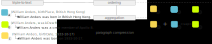
\includegraphics[width=\textwidth]{img/zeroshot_pipeline.pdf}
    \caption{A scheme of our pipeline for zero-shot data-to-text generation from RDF triples: (1) ordering, (2) aggregation, (3) paragraph compression. Individual pipeline modules are trained on a large general-domain text corpus and operate over text in natural language. In-domain knowledge is included only in the simple hand-crafted templates for each predicate.}\label{fig:zeroshot:pipeline}
\end{figure}



\subsection{Experiments}
\label{sec:pipeline-exp}
